\documentclass[twoside]{book}

% Packages required by doxygen
\usepackage{fixltx2e}
\usepackage{calc}
\usepackage{doxygen}
\usepackage[export]{adjustbox} % also loads graphicx
\usepackage{graphicx}
\usepackage[utf8]{inputenc}
\usepackage{makeidx}
\usepackage{multicol}
\usepackage{multirow}
\PassOptionsToPackage{warn}{textcomp}
\usepackage{textcomp}
\usepackage[nointegrals]{wasysym}
\usepackage[table]{xcolor}

% Font selection
\usepackage[T1]{fontenc}
\usepackage[scaled=.90]{helvet}
\usepackage{courier}
\usepackage{amssymb}
\usepackage{sectsty}
\renewcommand{\familydefault}{\sfdefault}
\allsectionsfont{%
  \fontseries{bc}\selectfont%
  \color{darkgray}%
}
\renewcommand{\DoxyLabelFont}{%
  \fontseries{bc}\selectfont%
  \color{darkgray}%
}
\newcommand{\+}{\discretionary{\mbox{\scriptsize$\hookleftarrow$}}{}{}}

% Page & text layout
\usepackage{geometry}
\geometry{%
  a4paper,%
  top=2.5cm,%
  bottom=2.5cm,%
  left=2.5cm,%
  right=2.5cm%
}
\tolerance=750
\hfuzz=15pt
\hbadness=750
\setlength{\emergencystretch}{15pt}
\setlength{\parindent}{0cm}
\setlength{\parskip}{3ex plus 2ex minus 2ex}
\makeatletter
\renewcommand{\paragraph}{%
  \@startsection{paragraph}{4}{0ex}{-1.0ex}{1.0ex}{%
    \normalfont\normalsize\bfseries\SS@parafont%
  }%
}
\renewcommand{\subparagraph}{%
  \@startsection{subparagraph}{5}{0ex}{-1.0ex}{1.0ex}{%
    \normalfont\normalsize\bfseries\SS@subparafont%
  }%
}
\makeatother

% Headers & footers
\usepackage{fancyhdr}
\pagestyle{fancyplain}
\fancyhead[LE]{\fancyplain{}{\bfseries\thepage}}
\fancyhead[CE]{\fancyplain{}{}}
\fancyhead[RE]{\fancyplain{}{\bfseries\leftmark}}
\fancyhead[LO]{\fancyplain{}{\bfseries\rightmark}}
\fancyhead[CO]{\fancyplain{}{}}
\fancyhead[RO]{\fancyplain{}{\bfseries\thepage}}
\fancyfoot[LE]{\fancyplain{}{}}
\fancyfoot[CE]{\fancyplain{}{}}
\fancyfoot[RE]{\fancyplain{}{\bfseries\scriptsize Generated by Doxygen }}
\fancyfoot[LO]{\fancyplain{}{\bfseries\scriptsize Generated by Doxygen }}
\fancyfoot[CO]{\fancyplain{}{}}
\fancyfoot[RO]{\fancyplain{}{}}
\renewcommand{\footrulewidth}{0.4pt}
\renewcommand{\chaptermark}[1]{%
  \markboth{#1}{}%
}
\renewcommand{\sectionmark}[1]{%
  \markright{\thesection\ #1}%
}

% Indices & bibliography
\usepackage{natbib}
\usepackage[titles]{tocloft}
\setcounter{tocdepth}{3}
\setcounter{secnumdepth}{5}
\makeindex

% Hyperlinks (required, but should be loaded last)
\usepackage{ifpdf}
\ifpdf
  \usepackage[pdftex,pagebackref=true]{hyperref}
\else
  \usepackage[ps2pdf,pagebackref=true]{hyperref}
\fi
\hypersetup{%
  colorlinks=true,%
  linkcolor=blue,%
  citecolor=blue,%
  unicode%
}

% Custom commands
\newcommand{\clearemptydoublepage}{%
  \newpage{\pagestyle{empty}\cleardoublepage}%
}

\usepackage{caption}
\captionsetup{labelsep=space,justification=centering,font={bf},singlelinecheck=off,skip=4pt,position=top}

%===== C O N T E N T S =====

\begin{document}

% Titlepage & ToC
\hypersetup{pageanchor=false,
             bookmarksnumbered=true,
             pdfencoding=unicode
            }
\pagenumbering{alph}
\begin{titlepage}
\vspace*{7cm}
\begin{center}%
{\Large Smeshalist }\\
\vspace*{1cm}
{\large Generated by Doxygen 1.8.12}\\
\end{center}
\end{titlepage}
\clearemptydoublepage
\pagenumbering{roman}
\tableofcontents
\clearemptydoublepage
\pagenumbering{arabic}
\hypersetup{pageanchor=true}

%--- Begin generated contents ---
\chapter{Hierarchical Index}
\section{Class Hierarchy}
This inheritance list is sorted roughly, but not completely, alphabetically\+:\begin{DoxyCompactList}
\item \contentsline{section}{Abstract\+Communiation}{\pageref{class_abstract_communiation}}{}
\begin{DoxyCompactList}
\item \contentsline{section}{Linux\+Communication}{\pageref{class_linux_communication}}{}
\item \contentsline{section}{Windows\+Communication}{\pageref{class_windows_communication}}{}
\end{DoxyCompactList}
\item \contentsline{section}{Geometry}{\pageref{class_geometry}}{}
\begin{DoxyCompactList}
\item \contentsline{section}{Block}{\pageref{class_block}}{}
\item \contentsline{section}{Edge}{\pageref{class_edge}}{}
\item \contentsline{section}{Face}{\pageref{class_face}}{}
\item \contentsline{section}{Point3D}{\pageref{class_point3_d}}{}
\item \contentsline{section}{Vertex}{\pageref{class_vertex}}{}
\end{DoxyCompactList}
\item \contentsline{section}{Smeshalist}{\pageref{class_smeshalist}}{}
\end{DoxyCompactList}

\chapter{Class Index}
\section{Class List}
Here are the classes, structs, unions and interfaces with brief descriptions\+:\begin{DoxyCompactList}
\item\contentsline{section}{\hyperlink{class_abstract_communiation}{Abstract\+Communiation} }{\pageref{class_abstract_communiation}}{}
\item\contentsline{section}{\hyperlink{class_block}{Block} }{\pageref{class_block}}{}
\item\contentsline{section}{\hyperlink{class_edge}{Edge} }{\pageref{class_edge}}{}
\item\contentsline{section}{\hyperlink{class_face}{Face} }{\pageref{class_face}}{}
\item\contentsline{section}{\hyperlink{class_geometry}{Geometry} }{\pageref{class_geometry}}{}
\item\contentsline{section}{\hyperlink{class_linux_communication}{Linux\+Communication} }{\pageref{class_linux_communication}}{}
\item\contentsline{section}{\hyperlink{class_point3_d}{Point3D} }{\pageref{class_point3_d}}{}
\item\contentsline{section}{\hyperlink{class_smeshalist}{Smeshalist} }{\pageref{class_smeshalist}}{}
\item\contentsline{section}{\hyperlink{class_vertex}{Vertex} }{\pageref{class_vertex}}{}
\item\contentsline{section}{\hyperlink{class_windows_communication}{Windows\+Communication} }{\pageref{class_windows_communication}}{}
\end{DoxyCompactList}

\chapter{Class Documentation}
\hypertarget{class_abstract_communiation}{}\section{Abstract\+Communiation Class Reference}
\label{class_abstract_communiation}\index{Abstract\+Communiation@{Abstract\+Communiation}}
Inheritance diagram for Abstract\+Communiation\+:\begin{figure}[H]
\begin{center}
\leavevmode
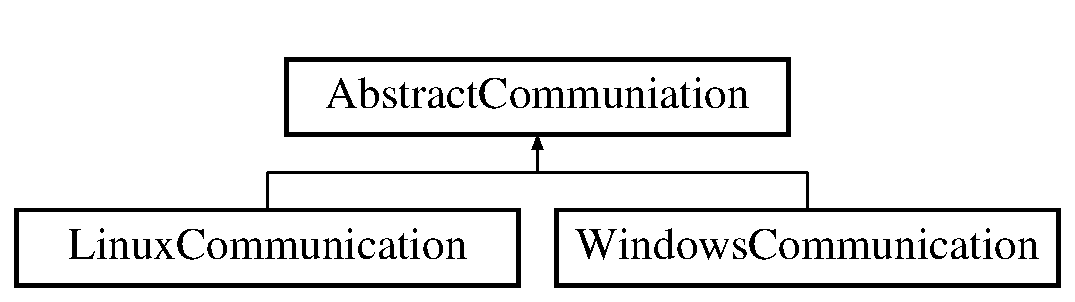
\includegraphics[height=2.000000cm]{class_abstract_communiation}
\end{center}
\end{figure}
\subsection*{Public Member Functions}
\begin{DoxyCompactItemize}
\item 
\hypertarget{class_abstract_communiation_ac34543a5061fd72060be1f07154bf63f}{}\label{class_abstract_communiation_ac34543a5061fd72060be1f07154bf63f} 
{\bfseries Abstract\+Communiation} (int port\+\_\+number)
\item 
\hypertarget{class_abstract_communiation_a1b0a8e332e2a384d1cee015dabdaf6e3}{}\label{class_abstract_communiation_a1b0a8e332e2a384d1cee015dabdaf6e3} 
virtual void {\bfseries Setup\+Socket} ()=0
\item 
\hypertarget{class_abstract_communiation_a923e54025ed727117e2cfdd2b7a4d218}{}\label{class_abstract_communiation_a923e54025ed727117e2cfdd2b7a4d218} 
virtual void {\bfseries Cleanup\+Socket} ()=0
\item 
\hypertarget{class_abstract_communiation_a912ae3810fd73acd17b47dc8d17eacd6}{}\label{class_abstract_communiation_a912ae3810fd73acd17b47dc8d17eacd6} 
virtual int {\bfseries Send\+Bytes\+To\+Core} (const char $\ast$buffer, int buffer\+\_\+size) const =0
\item 
\hypertarget{class_abstract_communiation_a0ea1c0a2b2401aa136bd055eb12ab7c4}{}\label{class_abstract_communiation_a0ea1c0a2b2401aa136bd055eb12ab7c4} 
virtual int {\bfseries Get\+Bytes\+From\+Core} (char $\ast$buffer, int buffer\+\_\+size)=0
\end{DoxyCompactItemize}
\subsection*{Protected Attributes}
\begin{DoxyCompactItemize}
\item 
\hypertarget{class_abstract_communiation_ac7a6e918a8ce78c88b0db4117491d1c3}{}\label{class_abstract_communiation_ac7a6e918a8ce78c88b0db4117491d1c3} 
int {\bfseries core\+\_\+port}
\end{DoxyCompactItemize}


The documentation for this class was generated from the following file\+:\begin{DoxyCompactItemize}
\item 
include/Abstract\+Communication.\+h\end{DoxyCompactItemize}

\hypertarget{class_block}{}\section{Block Class Reference}
\label{class_block}\index{Block@{Block}}


{\ttfamily \#include $<$Geometry.\+h$>$}

Inheritance diagram for Block\+:\begin{figure}[H]
\begin{center}
\leavevmode
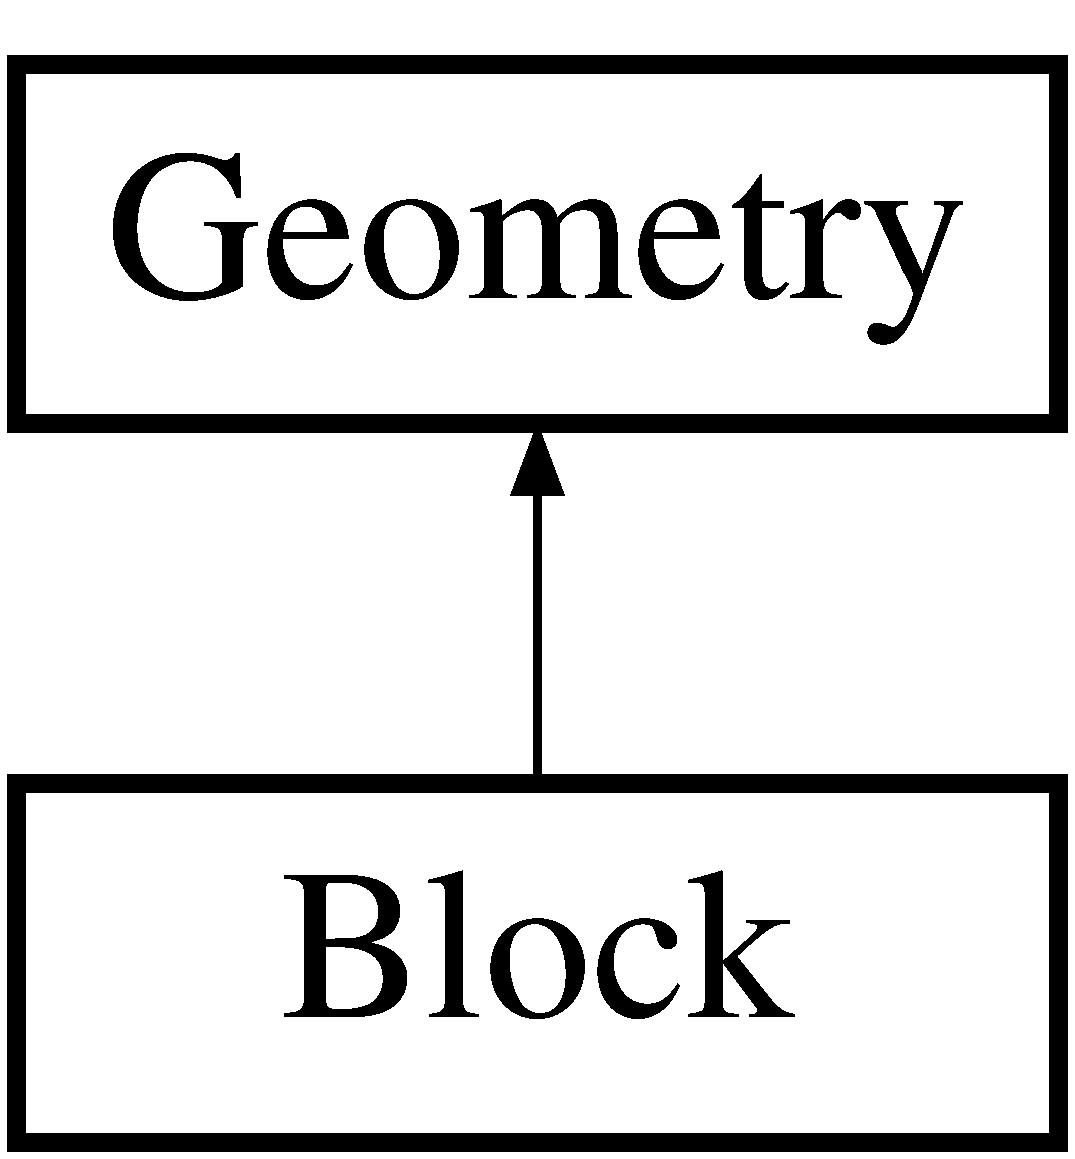
\includegraphics[height=2.000000cm]{class_block}
\end{center}
\end{figure}
\subsection*{Public Member Functions}
\begin{DoxyCompactItemize}
\item 
\hyperlink{class_block_a37658a946bf5067ad01d68d9ff086adc}{Block} ()
\item 
\hyperlink{class_block_acce9cf128eb5fec928a9172e529e777f}{Block} (\hyperlink{class_point3_d}{Point3D} v1, \hyperlink{class_point3_d}{Point3D} v2, \hyperlink{class_point3_d}{Point3D} v3, \hyperlink{class_point3_d}{Point3D} v4)
\item 
void \hyperlink{class_block_ab70b247a67e1adb3370943c8393d6077}{Set\+V1} (\hyperlink{class_point3_d}{Point3D} point)
\item 
void \hyperlink{class_block_a1ad1834202712fe4c67e1af5f7ccd7fd}{Set\+V2} (\hyperlink{class_point3_d}{Point3D} point)
\item 
void \hyperlink{class_block_a01d25d342ed145e454bf976b7be7e562}{Set\+V3} (\hyperlink{class_point3_d}{Point3D} point)
\item 
void \hyperlink{class_block_aba65bfccbd291227fda20d10d49ae345}{Set\+V4} (\hyperlink{class_point3_d}{Point3D} point)
\item 
\hyperlink{class_point3_d}{Point3D} \hyperlink{class_block_aaa48ffa0a41fafeb85fb05ad856dbcfe}{Get\+V1} () const
\item 
\hyperlink{class_point3_d}{Point3D} \hyperlink{class_block_aa5050e8dd9b471e1d6844e075d5c6171}{Get\+V2} () const
\item 
\hyperlink{class_point3_d}{Point3D} \hyperlink{class_block_af163578ec4cec1fdea035df72812f95b}{Get\+V3} () const
\item 
\hyperlink{class_point3_d}{Point3D} \hyperlink{class_block_a288e90a1b2e3fe8fb111e45fc93ab75b}{Get\+V4} () const
\end{DoxyCompactItemize}


\subsection{Detailed Description}
Class which provides internal application format for \textquotesingle{}block\textquotesingle{} structure. 

\subsection{Constructor \& Destructor Documentation}
\hypertarget{class_block_a37658a946bf5067ad01d68d9ff086adc}{}\label{class_block_a37658a946bf5067ad01d68d9ff086adc} 
\index{Block@{Block}!Block@{Block}}
\index{Block@{Block}!Block@{Block}}
\subsubsection{\texorpdfstring{Block()}{Block()}\hspace{0.1cm}{\footnotesize\ttfamily [1/2]}}
{\footnotesize\ttfamily Block\+::\+Block (\begin{DoxyParamCaption}{ }\end{DoxyParamCaption})}

Empty class constructor. \hypertarget{class_block_acce9cf128eb5fec928a9172e529e777f}{}\label{class_block_acce9cf128eb5fec928a9172e529e777f} 
\index{Block@{Block}!Block@{Block}}
\index{Block@{Block}!Block@{Block}}
\subsubsection{\texorpdfstring{Block()}{Block()}\hspace{0.1cm}{\footnotesize\ttfamily [2/2]}}
{\footnotesize\ttfamily Block\+::\+Block (\begin{DoxyParamCaption}\item[{\hyperlink{class_point3_d}{Point3D}}]{v1,  }\item[{\hyperlink{class_point3_d}{Point3D}}]{v2,  }\item[{\hyperlink{class_point3_d}{Point3D}}]{v3,  }\item[{\hyperlink{class_point3_d}{Point3D}}]{v4 }\end{DoxyParamCaption})}

Class constructor with \hyperlink{class_point3_d}{Point3D} arguments, representing points creating block. 
\begin{DoxyParams}{Parameters}
{\em v1} & first point creating block \\
\hline
{\em v2} & second point creating block \\
\hline
{\em v3} & third point creating block \\
\hline
{\em v3} & fourth point creating block \\
\hline
\end{DoxyParams}


\subsection{Member Function Documentation}
\hypertarget{class_block_aaa48ffa0a41fafeb85fb05ad856dbcfe}{}\label{class_block_aaa48ffa0a41fafeb85fb05ad856dbcfe} 
\index{Block@{Block}!Get\+V1@{Get\+V1}}
\index{Get\+V1@{Get\+V1}!Block@{Block}}
\subsubsection{\texorpdfstring{Get\+V1()}{GetV1()}}
{\footnotesize\ttfamily \hyperlink{class_point3_d}{Point3D} Block\+::\+Get\+V1 (\begin{DoxyParamCaption}{ }\end{DoxyParamCaption}) const}

Returns v1. \begin{DoxyReturn}{Returns}
first point creating block 
\end{DoxyReturn}
\hypertarget{class_block_aa5050e8dd9b471e1d6844e075d5c6171}{}\label{class_block_aa5050e8dd9b471e1d6844e075d5c6171} 
\index{Block@{Block}!Get\+V2@{Get\+V2}}
\index{Get\+V2@{Get\+V2}!Block@{Block}}
\subsubsection{\texorpdfstring{Get\+V2()}{GetV2()}}
{\footnotesize\ttfamily \hyperlink{class_point3_d}{Point3D} Block\+::\+Get\+V2 (\begin{DoxyParamCaption}{ }\end{DoxyParamCaption}) const}

Returns v2. \begin{DoxyReturn}{Returns}
second point creating block 
\end{DoxyReturn}
\hypertarget{class_block_af163578ec4cec1fdea035df72812f95b}{}\label{class_block_af163578ec4cec1fdea035df72812f95b} 
\index{Block@{Block}!Get\+V3@{Get\+V3}}
\index{Get\+V3@{Get\+V3}!Block@{Block}}
\subsubsection{\texorpdfstring{Get\+V3()}{GetV3()}}
{\footnotesize\ttfamily \hyperlink{class_point3_d}{Point3D} Block\+::\+Get\+V3 (\begin{DoxyParamCaption}{ }\end{DoxyParamCaption}) const}

Returns v3. \begin{DoxyReturn}{Returns}
third point creating block 
\end{DoxyReturn}
\hypertarget{class_block_a288e90a1b2e3fe8fb111e45fc93ab75b}{}\label{class_block_a288e90a1b2e3fe8fb111e45fc93ab75b} 
\index{Block@{Block}!Get\+V4@{Get\+V4}}
\index{Get\+V4@{Get\+V4}!Block@{Block}}
\subsubsection{\texorpdfstring{Get\+V4()}{GetV4()}}
{\footnotesize\ttfamily \hyperlink{class_point3_d}{Point3D} Block\+::\+Get\+V4 (\begin{DoxyParamCaption}{ }\end{DoxyParamCaption}) const}

Returns v4. \begin{DoxyReturn}{Returns}
fourth point creating block 
\end{DoxyReturn}
\hypertarget{class_block_ab70b247a67e1adb3370943c8393d6077}{}\label{class_block_ab70b247a67e1adb3370943c8393d6077} 
\index{Block@{Block}!Set\+V1@{Set\+V1}}
\index{Set\+V1@{Set\+V1}!Block@{Block}}
\subsubsection{\texorpdfstring{Set\+V1()}{SetV1()}}
{\footnotesize\ttfamily void Block\+::\+Set\+V1 (\begin{DoxyParamCaption}\item[{\hyperlink{class_point3_d}{Point3D}}]{point }\end{DoxyParamCaption})}

Method sets v1 field of the object. 
\begin{DoxyParams}{Parameters}
{\em point} & first point creating block \\
\hline
\end{DoxyParams}
\hypertarget{class_block_a1ad1834202712fe4c67e1af5f7ccd7fd}{}\label{class_block_a1ad1834202712fe4c67e1af5f7ccd7fd} 
\index{Block@{Block}!Set\+V2@{Set\+V2}}
\index{Set\+V2@{Set\+V2}!Block@{Block}}
\subsubsection{\texorpdfstring{Set\+V2()}{SetV2()}}
{\footnotesize\ttfamily void Block\+::\+Set\+V2 (\begin{DoxyParamCaption}\item[{\hyperlink{class_point3_d}{Point3D}}]{point }\end{DoxyParamCaption})}

Method sets v2 field of the object. 
\begin{DoxyParams}{Parameters}
{\em point} & second point creating block \\
\hline
\end{DoxyParams}
\hypertarget{class_block_a01d25d342ed145e454bf976b7be7e562}{}\label{class_block_a01d25d342ed145e454bf976b7be7e562} 
\index{Block@{Block}!Set\+V3@{Set\+V3}}
\index{Set\+V3@{Set\+V3}!Block@{Block}}
\subsubsection{\texorpdfstring{Set\+V3()}{SetV3()}}
{\footnotesize\ttfamily void Block\+::\+Set\+V3 (\begin{DoxyParamCaption}\item[{\hyperlink{class_point3_d}{Point3D}}]{point }\end{DoxyParamCaption})}

Method sets v3 field of the object. 
\begin{DoxyParams}{Parameters}
{\em point} & third point creating block \\
\hline
\end{DoxyParams}
\hypertarget{class_block_aba65bfccbd291227fda20d10d49ae345}{}\label{class_block_aba65bfccbd291227fda20d10d49ae345} 
\index{Block@{Block}!Set\+V4@{Set\+V4}}
\index{Set\+V4@{Set\+V4}!Block@{Block}}
\subsubsection{\texorpdfstring{Set\+V4()}{SetV4()}}
{\footnotesize\ttfamily void Block\+::\+Set\+V4 (\begin{DoxyParamCaption}\item[{\hyperlink{class_point3_d}{Point3D}}]{point }\end{DoxyParamCaption})}

Method sets v4 field of the object. 
\begin{DoxyParams}{Parameters}
{\em point} & fourth point creating block \\
\hline
\end{DoxyParams}


The documentation for this class was generated from the following file\+:\begin{DoxyCompactItemize}
\item 
include/Geometry.\+h\end{DoxyCompactItemize}

\hypertarget{class_edge}{}\section{Edge Class Reference}
\label{class_edge}\index{Edge@{Edge}}


{\ttfamily \#include $<$Geometry.\+h$>$}

Inheritance diagram for Edge\+:\begin{figure}[H]
\begin{center}
\leavevmode
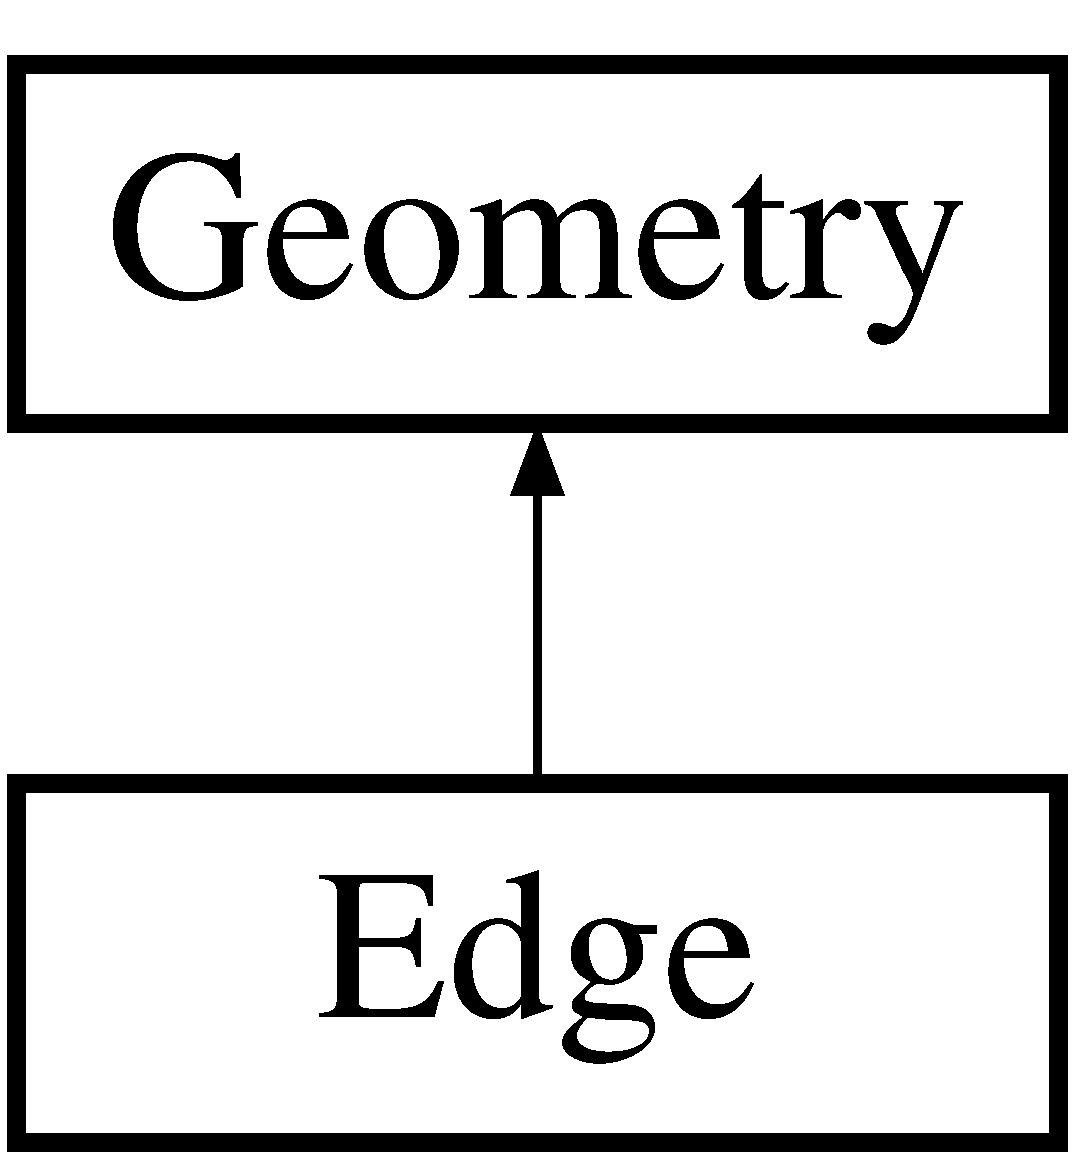
\includegraphics[height=2.000000cm]{class_edge}
\end{center}
\end{figure}
\subsection*{Public Member Functions}
\begin{DoxyCompactItemize}
\item 
\hyperlink{class_edge_a3106b11d60125009dbf7a738ce540fdf}{Edge} ()
\item 
\hyperlink{class_edge_a7011d5e767aad79a7c3798c297660a75}{Edge} (\hyperlink{class_point3_d}{Point3D} v1, \hyperlink{class_point3_d}{Point3D} v2)
\item 
void \hyperlink{class_edge_a3c7909c0d93258c05e61fb1704c699ec}{Set\+V1} (\hyperlink{class_point3_d}{Point3D} point)
\item 
void \hyperlink{class_edge_af89cb05e0c7d9cbf31330e445a5d0752}{Set\+V2} (\hyperlink{class_point3_d}{Point3D} point)
\item 
\hyperlink{class_point3_d}{Point3D} \hyperlink{class_edge_a770284695e38a15103cc04ef4e3a2ff9}{Get\+V1} () const
\item 
\hyperlink{class_point3_d}{Point3D} \hyperlink{class_edge_a9be2780962afac8b55848ea1df3a28e9}{Get\+V2} () const
\end{DoxyCompactItemize}


\subsection{Detailed Description}
Class which provides internal application format for \textquotesingle{}edge\textquotesingle{} structure. 

\subsection{Constructor \& Destructor Documentation}
\hypertarget{class_edge_a3106b11d60125009dbf7a738ce540fdf}{}\label{class_edge_a3106b11d60125009dbf7a738ce540fdf} 
\index{Edge@{Edge}!Edge@{Edge}}
\index{Edge@{Edge}!Edge@{Edge}}
\subsubsection{\texorpdfstring{Edge()}{Edge()}\hspace{0.1cm}{\footnotesize\ttfamily [1/2]}}
{\footnotesize\ttfamily Edge\+::\+Edge (\begin{DoxyParamCaption}{ }\end{DoxyParamCaption})}

Empty class constructor. \hypertarget{class_edge_a7011d5e767aad79a7c3798c297660a75}{}\label{class_edge_a7011d5e767aad79a7c3798c297660a75} 
\index{Edge@{Edge}!Edge@{Edge}}
\index{Edge@{Edge}!Edge@{Edge}}
\subsubsection{\texorpdfstring{Edge()}{Edge()}\hspace{0.1cm}{\footnotesize\ttfamily [2/2]}}
{\footnotesize\ttfamily Edge\+::\+Edge (\begin{DoxyParamCaption}\item[{\hyperlink{class_point3_d}{Point3D}}]{v1,  }\item[{\hyperlink{class_point3_d}{Point3D}}]{v2 }\end{DoxyParamCaption})}

Class constructor with \hyperlink{class_point3_d}{Point3D} arguments, representing two ends of edge. 
\begin{DoxyParams}{Parameters}
{\em v1} & point representing one end of edge \\
\hline
{\em v2} & point representing second end of edge \\
\hline
\end{DoxyParams}


\subsection{Member Function Documentation}
\hypertarget{class_edge_a770284695e38a15103cc04ef4e3a2ff9}{}\label{class_edge_a770284695e38a15103cc04ef4e3a2ff9} 
\index{Edge@{Edge}!Get\+V1@{Get\+V1}}
\index{Get\+V1@{Get\+V1}!Edge@{Edge}}
\subsubsection{\texorpdfstring{Get\+V1()}{GetV1()}}
{\footnotesize\ttfamily \hyperlink{class_point3_d}{Point3D} Edge\+::\+Get\+V1 (\begin{DoxyParamCaption}{ }\end{DoxyParamCaption}) const}

Returns v1. \begin{DoxyReturn}{Returns}
point representing one end of edge 
\end{DoxyReturn}
\hypertarget{class_edge_a9be2780962afac8b55848ea1df3a28e9}{}\label{class_edge_a9be2780962afac8b55848ea1df3a28e9} 
\index{Edge@{Edge}!Get\+V2@{Get\+V2}}
\index{Get\+V2@{Get\+V2}!Edge@{Edge}}
\subsubsection{\texorpdfstring{Get\+V2()}{GetV2()}}
{\footnotesize\ttfamily \hyperlink{class_point3_d}{Point3D} Edge\+::\+Get\+V2 (\begin{DoxyParamCaption}{ }\end{DoxyParamCaption}) const}

Returns v2. \begin{DoxyReturn}{Returns}
point representing second end of edge 
\end{DoxyReturn}
\hypertarget{class_edge_a3c7909c0d93258c05e61fb1704c699ec}{}\label{class_edge_a3c7909c0d93258c05e61fb1704c699ec} 
\index{Edge@{Edge}!Set\+V1@{Set\+V1}}
\index{Set\+V1@{Set\+V1}!Edge@{Edge}}
\subsubsection{\texorpdfstring{Set\+V1()}{SetV1()}}
{\footnotesize\ttfamily void Edge\+::\+Set\+V1 (\begin{DoxyParamCaption}\item[{\hyperlink{class_point3_d}{Point3D}}]{point }\end{DoxyParamCaption})}

Method sets v1 field of the object. 
\begin{DoxyParams}{Parameters}
{\em point} & point representing the one end of edge \\
\hline
\end{DoxyParams}
\hypertarget{class_edge_af89cb05e0c7d9cbf31330e445a5d0752}{}\label{class_edge_af89cb05e0c7d9cbf31330e445a5d0752} 
\index{Edge@{Edge}!Set\+V2@{Set\+V2}}
\index{Set\+V2@{Set\+V2}!Edge@{Edge}}
\subsubsection{\texorpdfstring{Set\+V2()}{SetV2()}}
{\footnotesize\ttfamily void Edge\+::\+Set\+V2 (\begin{DoxyParamCaption}\item[{\hyperlink{class_point3_d}{Point3D}}]{point }\end{DoxyParamCaption})}

Method sets v2 field of the object. 
\begin{DoxyParams}{Parameters}
{\em point} & point representing the second end of edge \\
\hline
\end{DoxyParams}


The documentation for this class was generated from the following file\+:\begin{DoxyCompactItemize}
\item 
include/Geometry.\+h\end{DoxyCompactItemize}

\hypertarget{class_face}{}\section{Face Class Reference}
\label{class_face}\index{Face@{Face}}


{\ttfamily \#include $<$Geometry.\+h$>$}

Inheritance diagram for Face\+:\begin{figure}[H]
\begin{center}
\leavevmode
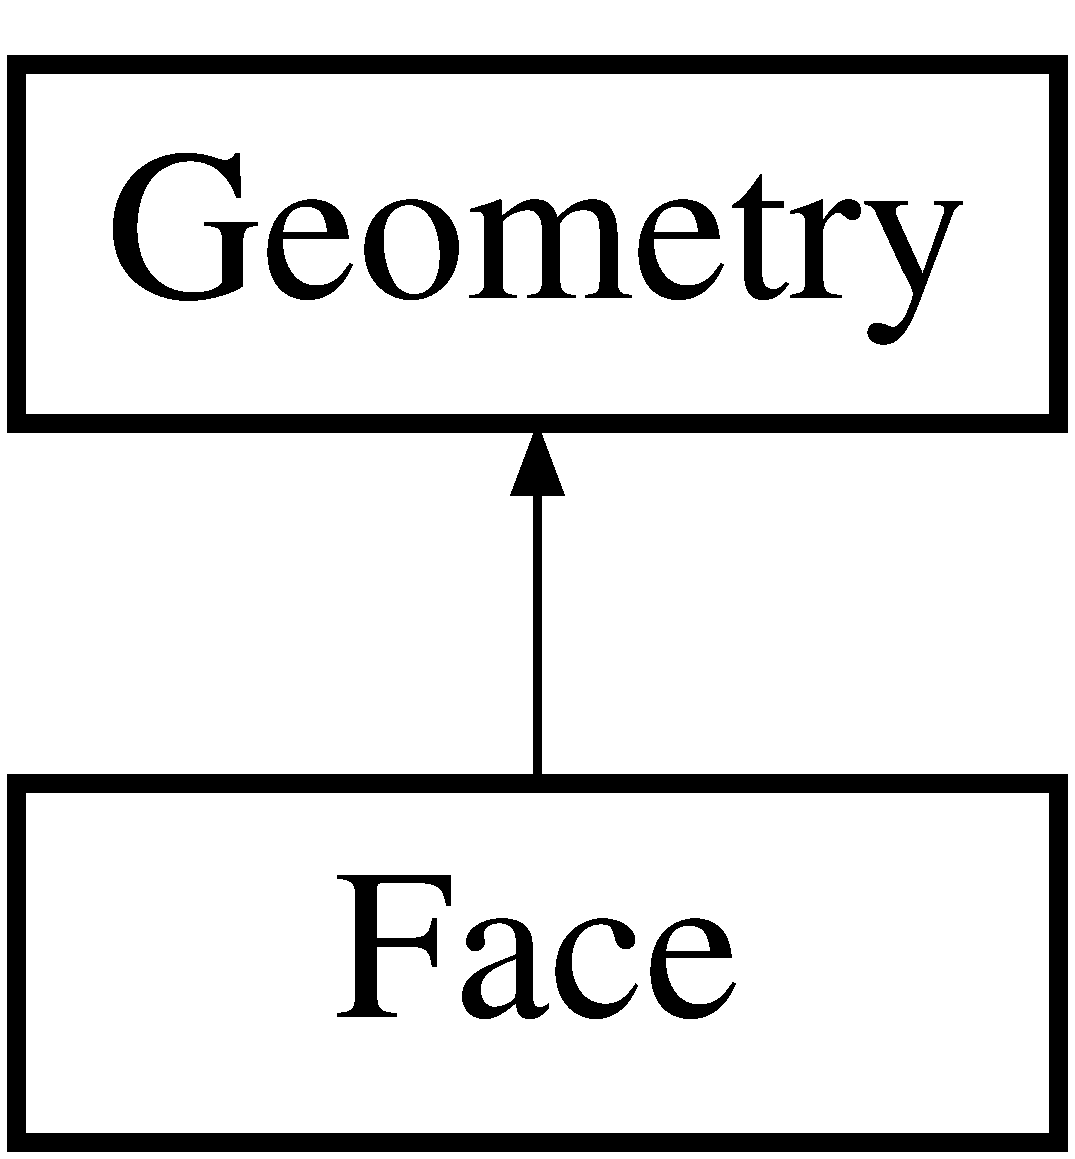
\includegraphics[height=2.000000cm]{class_face}
\end{center}
\end{figure}
\subsection*{Public Member Functions}
\begin{DoxyCompactItemize}
\item 
\hyperlink{class_face_afdb634bc2d5287ba0d62e46b57e9dc2e}{Face} ()
\item 
\hyperlink{class_face_aaf867e5f898344930188a82a566b1a55}{Face} (\hyperlink{class_point3_d}{Point3D} v1, \hyperlink{class_point3_d}{Point3D} v2, \hyperlink{class_point3_d}{Point3D} v3)
\item 
void \hyperlink{class_face_a0aa6787b68f53915e9638eff3b32f6db}{Set\+V1} (\hyperlink{class_point3_d}{Point3D} point)
\item 
void \hyperlink{class_face_ad4cd189f6de7169d1b7d256fc76836e7}{Set\+V2} (\hyperlink{class_point3_d}{Point3D} point)
\item 
void \hyperlink{class_face_a81311d36d3f1bb6f7b92629c327a06aa}{Set\+V3} (\hyperlink{class_point3_d}{Point3D} point)
\item 
\hyperlink{class_point3_d}{Point3D} \hyperlink{class_face_ae6df8ea5ce4f2b7b6a5ad1dcc6fb4d07}{Get\+V1} () const
\item 
\hyperlink{class_point3_d}{Point3D} \hyperlink{class_face_a8ce9ccf7617c5d7224d885c08cf8651e}{Get\+V2} () const
\item 
\hyperlink{class_point3_d}{Point3D} \hyperlink{class_face_a8aaddb9ebb59e71a21df96e6d38fe29d}{Get\+V3} () const
\end{DoxyCompactItemize}


\subsection{Detailed Description}
Class which provides internal application format for \textquotesingle{}face\textquotesingle{} structure. 

\subsection{Constructor \& Destructor Documentation}
\hypertarget{class_face_afdb634bc2d5287ba0d62e46b57e9dc2e}{}\label{class_face_afdb634bc2d5287ba0d62e46b57e9dc2e} 
\index{Face@{Face}!Face@{Face}}
\index{Face@{Face}!Face@{Face}}
\subsubsection{\texorpdfstring{Face()}{Face()}\hspace{0.1cm}{\footnotesize\ttfamily [1/2]}}
{\footnotesize\ttfamily Face\+::\+Face (\begin{DoxyParamCaption}{ }\end{DoxyParamCaption})}

Empty class constructor. \hypertarget{class_face_aaf867e5f898344930188a82a566b1a55}{}\label{class_face_aaf867e5f898344930188a82a566b1a55} 
\index{Face@{Face}!Face@{Face}}
\index{Face@{Face}!Face@{Face}}
\subsubsection{\texorpdfstring{Face()}{Face()}\hspace{0.1cm}{\footnotesize\ttfamily [2/2]}}
{\footnotesize\ttfamily Face\+::\+Face (\begin{DoxyParamCaption}\item[{\hyperlink{class_point3_d}{Point3D}}]{v1,  }\item[{\hyperlink{class_point3_d}{Point3D}}]{v2,  }\item[{\hyperlink{class_point3_d}{Point3D}}]{v3 }\end{DoxyParamCaption})}

Class constructor with \hyperlink{class_point3_d}{Point3D} arguments, representing points creating face. 
\begin{DoxyParams}{Parameters}
{\em v1} & first point creating face \\
\hline
{\em v2} & second point creating face \\
\hline
{\em v3} & third point creating face \\
\hline
\end{DoxyParams}


\subsection{Member Function Documentation}
\hypertarget{class_face_ae6df8ea5ce4f2b7b6a5ad1dcc6fb4d07}{}\label{class_face_ae6df8ea5ce4f2b7b6a5ad1dcc6fb4d07} 
\index{Face@{Face}!Get\+V1@{Get\+V1}}
\index{Get\+V1@{Get\+V1}!Face@{Face}}
\subsubsection{\texorpdfstring{Get\+V1()}{GetV1()}}
{\footnotesize\ttfamily \hyperlink{class_point3_d}{Point3D} Face\+::\+Get\+V1 (\begin{DoxyParamCaption}{ }\end{DoxyParamCaption}) const}

Returns v1. \begin{DoxyReturn}{Returns}
first point creating face 
\end{DoxyReturn}
\hypertarget{class_face_a8ce9ccf7617c5d7224d885c08cf8651e}{}\label{class_face_a8ce9ccf7617c5d7224d885c08cf8651e} 
\index{Face@{Face}!Get\+V2@{Get\+V2}}
\index{Get\+V2@{Get\+V2}!Face@{Face}}
\subsubsection{\texorpdfstring{Get\+V2()}{GetV2()}}
{\footnotesize\ttfamily \hyperlink{class_point3_d}{Point3D} Face\+::\+Get\+V2 (\begin{DoxyParamCaption}{ }\end{DoxyParamCaption}) const}

Returns v2. \begin{DoxyReturn}{Returns}
second point creating face 
\end{DoxyReturn}
\hypertarget{class_face_a8aaddb9ebb59e71a21df96e6d38fe29d}{}\label{class_face_a8aaddb9ebb59e71a21df96e6d38fe29d} 
\index{Face@{Face}!Get\+V3@{Get\+V3}}
\index{Get\+V3@{Get\+V3}!Face@{Face}}
\subsubsection{\texorpdfstring{Get\+V3()}{GetV3()}}
{\footnotesize\ttfamily \hyperlink{class_point3_d}{Point3D} Face\+::\+Get\+V3 (\begin{DoxyParamCaption}{ }\end{DoxyParamCaption}) const}

Returns v3. \begin{DoxyReturn}{Returns}
third point creating face 
\end{DoxyReturn}
\hypertarget{class_face_a0aa6787b68f53915e9638eff3b32f6db}{}\label{class_face_a0aa6787b68f53915e9638eff3b32f6db} 
\index{Face@{Face}!Set\+V1@{Set\+V1}}
\index{Set\+V1@{Set\+V1}!Face@{Face}}
\subsubsection{\texorpdfstring{Set\+V1()}{SetV1()}}
{\footnotesize\ttfamily void Face\+::\+Set\+V1 (\begin{DoxyParamCaption}\item[{\hyperlink{class_point3_d}{Point3D}}]{point }\end{DoxyParamCaption})}

Method sets v1 field of the object. 
\begin{DoxyParams}{Parameters}
{\em point} & first point creating face \\
\hline
\end{DoxyParams}
\hypertarget{class_face_ad4cd189f6de7169d1b7d256fc76836e7}{}\label{class_face_ad4cd189f6de7169d1b7d256fc76836e7} 
\index{Face@{Face}!Set\+V2@{Set\+V2}}
\index{Set\+V2@{Set\+V2}!Face@{Face}}
\subsubsection{\texorpdfstring{Set\+V2()}{SetV2()}}
{\footnotesize\ttfamily void Face\+::\+Set\+V2 (\begin{DoxyParamCaption}\item[{\hyperlink{class_point3_d}{Point3D}}]{point }\end{DoxyParamCaption})}

Method sets v2 field of the object. 
\begin{DoxyParams}{Parameters}
{\em point} & second point creating face \\
\hline
\end{DoxyParams}
\hypertarget{class_face_a81311d36d3f1bb6f7b92629c327a06aa}{}\label{class_face_a81311d36d3f1bb6f7b92629c327a06aa} 
\index{Face@{Face}!Set\+V3@{Set\+V3}}
\index{Set\+V3@{Set\+V3}!Face@{Face}}
\subsubsection{\texorpdfstring{Set\+V3()}{SetV3()}}
{\footnotesize\ttfamily void Face\+::\+Set\+V3 (\begin{DoxyParamCaption}\item[{\hyperlink{class_point3_d}{Point3D}}]{point }\end{DoxyParamCaption})}

Method sets v3 field of the object. 
\begin{DoxyParams}{Parameters}
{\em point} & third point creating face \\
\hline
\end{DoxyParams}


The documentation for this class was generated from the following file\+:\begin{DoxyCompactItemize}
\item 
include/Geometry.\+h\end{DoxyCompactItemize}

\hypertarget{class_geometry}{}\section{Geometry Class Reference}
\label{class_geometry}\index{Geometry@{Geometry}}


{\ttfamily \#include $<$Geometry.\+h$>$}

Inheritance diagram for Geometry\+:\begin{figure}[H]
\begin{center}
\leavevmode
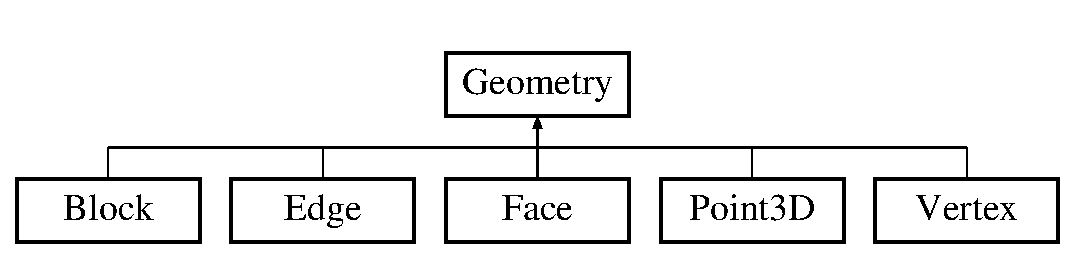
\includegraphics[height=2.000000cm]{class_geometry}
\end{center}
\end{figure}
\subsection*{Public Member Functions}
\begin{DoxyCompactItemize}
\item 
void \hyperlink{class_geometry_a79fca7521afb70ed250bc397786f453a}{Set\+Quality} (double q)
\item 
double \hyperlink{class_geometry_a1133070c22222662eb75f92a0dcf1843}{Get\+Quality} () const
\item 
void \hyperlink{class_geometry_a311538e128f84a532d1a63d44843f33d}{Set\+Group\+Id} (int id)
\item 
int \hyperlink{class_geometry_a0edac5bbf074cb985207dbb50e62821a}{Get\+Group\+Id} () const
\item 
void \hyperlink{class_geometry_aae7622e0d7dedc29426a671745837101}{Set\+Label} (string l)
\item 
string \hyperlink{class_geometry_a790bc03456ac9c225a004ebfb9279487}{Get\+Label} () const
\end{DoxyCompactItemize}


\subsection{Detailed Description}
Base class of all geometry classes. It holds all the geometry\textquotesingle{}s properties. 

\subsection{Member Function Documentation}
\hypertarget{class_geometry_a0edac5bbf074cb985207dbb50e62821a}{}\label{class_geometry_a0edac5bbf074cb985207dbb50e62821a} 
\index{Geometry@{Geometry}!Get\+Group\+Id@{Get\+Group\+Id}}
\index{Get\+Group\+Id@{Get\+Group\+Id}!Geometry@{Geometry}}
\subsubsection{\texorpdfstring{Get\+Group\+Id()}{GetGroupId()}}
{\footnotesize\ttfamily int Geometry\+::\+Get\+Group\+Id (\begin{DoxyParamCaption}{ }\end{DoxyParamCaption}) const}

Returns value of geometry\textquotesingle{}s group\+\_\+id property. \begin{DoxyReturn}{Returns}
value of group\+\_\+id property 
\end{DoxyReturn}
\hypertarget{class_geometry_a790bc03456ac9c225a004ebfb9279487}{}\label{class_geometry_a790bc03456ac9c225a004ebfb9279487} 
\index{Geometry@{Geometry}!Get\+Label@{Get\+Label}}
\index{Get\+Label@{Get\+Label}!Geometry@{Geometry}}
\subsubsection{\texorpdfstring{Get\+Label()}{GetLabel()}}
{\footnotesize\ttfamily string Geometry\+::\+Get\+Label (\begin{DoxyParamCaption}{ }\end{DoxyParamCaption}) const}

Returns geometry\textquotesingle{}s label. \begin{DoxyReturn}{Returns}
geometry\textquotesingle{}s label 
\end{DoxyReturn}
\hypertarget{class_geometry_a1133070c22222662eb75f92a0dcf1843}{}\label{class_geometry_a1133070c22222662eb75f92a0dcf1843} 
\index{Geometry@{Geometry}!Get\+Quality@{Get\+Quality}}
\index{Get\+Quality@{Get\+Quality}!Geometry@{Geometry}}
\subsubsection{\texorpdfstring{Get\+Quality()}{GetQuality()}}
{\footnotesize\ttfamily double Geometry\+::\+Get\+Quality (\begin{DoxyParamCaption}{ }\end{DoxyParamCaption}) const}

Returns value of geometry\textquotesingle{}s quality property. \begin{DoxyReturn}{Returns}
value of quality property 
\end{DoxyReturn}
\hypertarget{class_geometry_a311538e128f84a532d1a63d44843f33d}{}\label{class_geometry_a311538e128f84a532d1a63d44843f33d} 
\index{Geometry@{Geometry}!Set\+Group\+Id@{Set\+Group\+Id}}
\index{Set\+Group\+Id@{Set\+Group\+Id}!Geometry@{Geometry}}
\subsubsection{\texorpdfstring{Set\+Group\+Id()}{SetGroupId()}}
{\footnotesize\ttfamily void Geometry\+::\+Set\+Group\+Id (\begin{DoxyParamCaption}\item[{int}]{id }\end{DoxyParamCaption})}

Sets the group\+\_\+id property. 
\begin{DoxyParams}{Parameters}
{\em id} & value to be set \\
\hline
\end{DoxyParams}
\hypertarget{class_geometry_aae7622e0d7dedc29426a671745837101}{}\label{class_geometry_aae7622e0d7dedc29426a671745837101} 
\index{Geometry@{Geometry}!Set\+Label@{Set\+Label}}
\index{Set\+Label@{Set\+Label}!Geometry@{Geometry}}
\subsubsection{\texorpdfstring{Set\+Label()}{SetLabel()}}
{\footnotesize\ttfamily void Geometry\+::\+Set\+Label (\begin{DoxyParamCaption}\item[{string}]{l }\end{DoxyParamCaption})}

Sets the label of geometry. 
\begin{DoxyParams}{Parameters}
{\em l} & string containing label to be set \\
\hline
\end{DoxyParams}
\hypertarget{class_geometry_a79fca7521afb70ed250bc397786f453a}{}\label{class_geometry_a79fca7521afb70ed250bc397786f453a} 
\index{Geometry@{Geometry}!Set\+Quality@{Set\+Quality}}
\index{Set\+Quality@{Set\+Quality}!Geometry@{Geometry}}
\subsubsection{\texorpdfstring{Set\+Quality()}{SetQuality()}}
{\footnotesize\ttfamily void Geometry\+::\+Set\+Quality (\begin{DoxyParamCaption}\item[{double}]{q }\end{DoxyParamCaption})}

Sets the quality property. 
\begin{DoxyParams}{Parameters}
{\em q} & value to be set \\
\hline
\end{DoxyParams}


The documentation for this class was generated from the following file\+:\begin{DoxyCompactItemize}
\item 
include/Geometry.\+h\end{DoxyCompactItemize}

\hypertarget{class_linux_communication}{}\section{Linux\+Communication Class Reference}
\label{class_linux_communication}\index{Linux\+Communication@{Linux\+Communication}}
Inheritance diagram for Linux\+Communication\+:\begin{figure}[H]
\begin{center}
\leavevmode
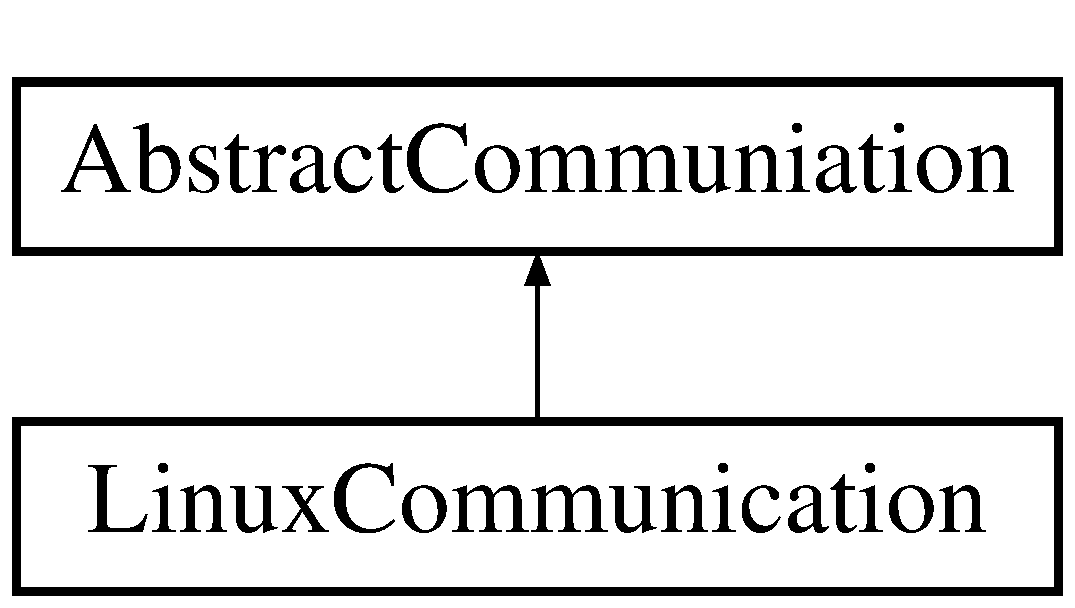
\includegraphics[height=2.000000cm]{class_linux_communication}
\end{center}
\end{figure}
\subsection*{Public Member Functions}
\begin{DoxyCompactItemize}
\item 
\hypertarget{class_linux_communication_ab18ccae5958d77b1e1a51b19ac5ff875}{}\label{class_linux_communication_ab18ccae5958d77b1e1a51b19ac5ff875} 
{\bfseries Linux\+Communication} (int port\+\_\+number)
\item 
\hypertarget{class_linux_communication_ac73a679c9601fc3f59ad572306f6ea11}{}\label{class_linux_communication_ac73a679c9601fc3f59ad572306f6ea11} 
void {\bfseries Setup\+Socket} ()
\item 
\hypertarget{class_linux_communication_a65fde2bd6e4000977ff38a2c8e49808b}{}\label{class_linux_communication_a65fde2bd6e4000977ff38a2c8e49808b} 
void {\bfseries Cleanup\+Socket} ()
\item 
\hypertarget{class_linux_communication_a2caae46991804776d4504811a1a31b86}{}\label{class_linux_communication_a2caae46991804776d4504811a1a31b86} 
int {\bfseries Send\+Bytes\+To\+Core} (const char $\ast$buffer, int buffer\+\_\+size) const
\item 
\hypertarget{class_linux_communication_aea3499292cf3d7fec441c2b88f7f5d1a}{}\label{class_linux_communication_aea3499292cf3d7fec441c2b88f7f5d1a} 
int {\bfseries Get\+Bytes\+From\+Core} (char $\ast$buffer, int buffer\+\_\+size)
\end{DoxyCompactItemize}
\subsection*{Additional Inherited Members}


The documentation for this class was generated from the following file\+:\begin{DoxyCompactItemize}
\item 
include/Linux\+Communication.\+h\end{DoxyCompactItemize}

\hypertarget{class_point3_d}{}\section{Point3D Class Reference}
\label{class_point3_d}\index{Point3D@{Point3D}}


{\ttfamily \#include $<$Geometry.\+h$>$}

Inheritance diagram for Point3D\+:\begin{figure}[H]
\begin{center}
\leavevmode
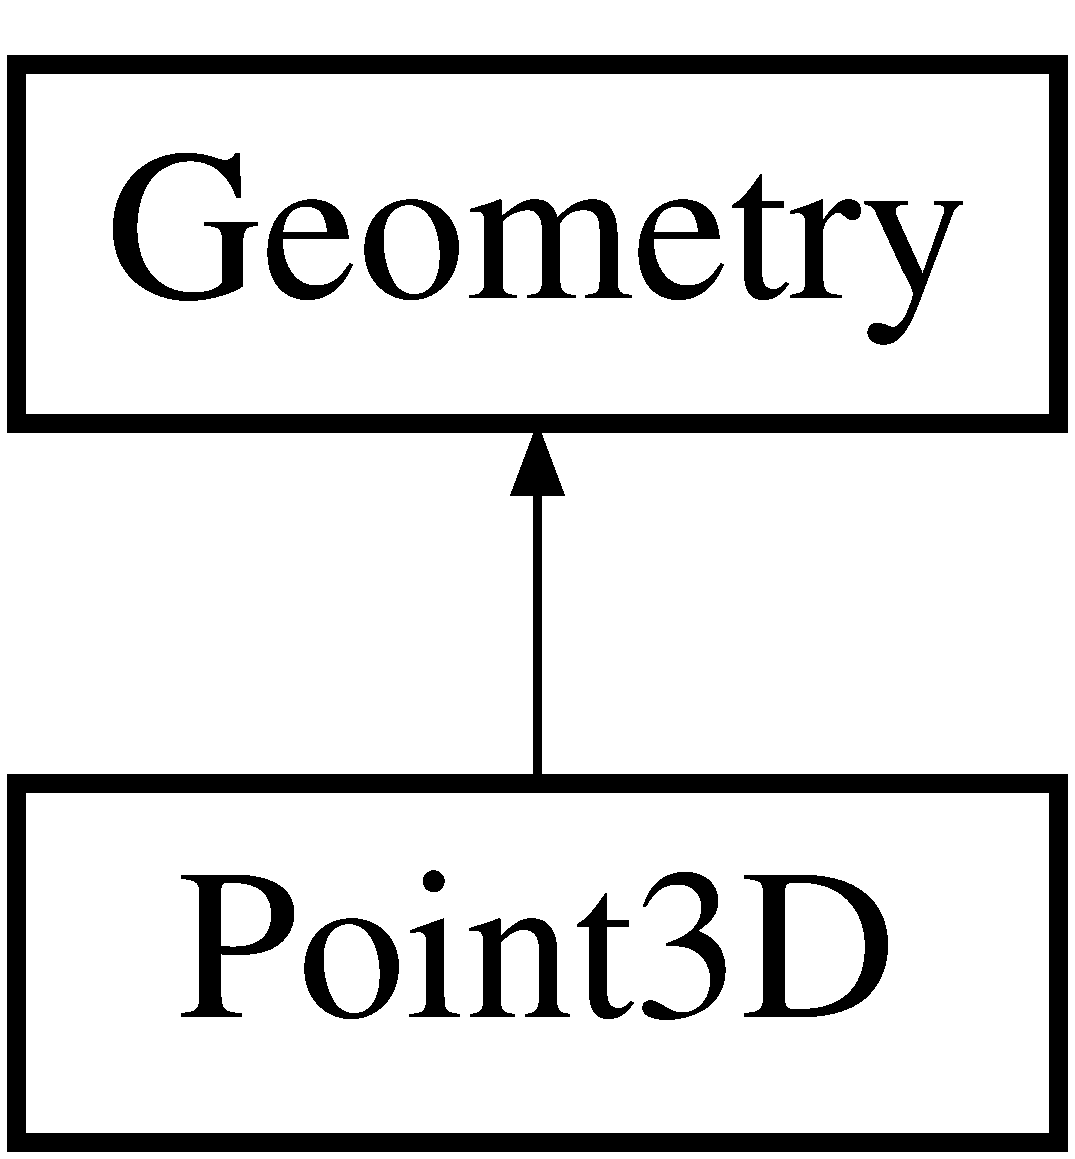
\includegraphics[height=2.000000cm]{class_point3_d}
\end{center}
\end{figure}
\subsection*{Public Member Functions}
\begin{DoxyCompactItemize}
\item 
\hyperlink{class_point3_d_a0e7bbbad6dc4316a9e17d9c4d17c8016}{Point3D} ()
\item 
\hyperlink{class_point3_d_a4ab689160e40d1052d18d4eb96b37419}{Point3D} (double x, double y, double z)
\item 
\hyperlink{class_point3_d_abb578ef0a4d869c60518d03c2850bc86}{Point3D} (double x, double y)
\item 
void \hyperlink{class_point3_d_a49f776d3cf82882d8ea1971cea9ffda3}{SetX} (double value)
\item 
void \hyperlink{class_point3_d_a7d770b248d505057a7ef5c59092ab1e3}{SetY} (double value)
\item 
void \hyperlink{class_point3_d_a2f7667f3e19b8ac1335f50794232a2c5}{SetZ} (double value)
\item 
double \hyperlink{class_point3_d_a38cf0869ef4de11a4f02ad65513c1a4e}{GetX} () const
\item 
double \hyperlink{class_point3_d_a9e0e1e5926240f6ba9a4676586bd574c}{GetY} () const
\item 
double \hyperlink{class_point3_d_af6eb3e13adb7057a54b34a973d430162}{GetZ} () const
\end{DoxyCompactItemize}


\subsection{Detailed Description}
Class which stores point coordinates. All other structure objects from \hyperlink{_geometry_8h_source}{Geometry.\+h} use one or more \hyperlink{class_point3_d}{Point3D} objects to build the structure. 

\subsection{Constructor \& Destructor Documentation}
\hypertarget{class_point3_d_a0e7bbbad6dc4316a9e17d9c4d17c8016}{}\label{class_point3_d_a0e7bbbad6dc4316a9e17d9c4d17c8016} 
\index{Point3D@{Point3D}!Point3D@{Point3D}}
\index{Point3D@{Point3D}!Point3D@{Point3D}}
\subsubsection{\texorpdfstring{Point3\+D()}{Point3D()}\hspace{0.1cm}{\footnotesize\ttfamily [1/3]}}
{\footnotesize\ttfamily Point3\+D\+::\+Point3D (\begin{DoxyParamCaption}{ }\end{DoxyParamCaption})}

Empty class constructor. \hypertarget{class_point3_d_a4ab689160e40d1052d18d4eb96b37419}{}\label{class_point3_d_a4ab689160e40d1052d18d4eb96b37419} 
\index{Point3D@{Point3D}!Point3D@{Point3D}}
\index{Point3D@{Point3D}!Point3D@{Point3D}}
\subsubsection{\texorpdfstring{Point3\+D()}{Point3D()}\hspace{0.1cm}{\footnotesize\ttfamily [2/3]}}
{\footnotesize\ttfamily Point3\+D\+::\+Point3D (\begin{DoxyParamCaption}\item[{double}]{x,  }\item[{double}]{y,  }\item[{double}]{z }\end{DoxyParamCaption})}

Class constructor. 
\begin{DoxyParams}{Parameters}
{\em x} & the x coordinate \\
\hline
{\em y} & the y coordinate \\
\hline
{\em z} & the z coordinate \\
\hline
\end{DoxyParams}
\hypertarget{class_point3_d_abb578ef0a4d869c60518d03c2850bc86}{}\label{class_point3_d_abb578ef0a4d869c60518d03c2850bc86} 
\index{Point3D@{Point3D}!Point3D@{Point3D}}
\index{Point3D@{Point3D}!Point3D@{Point3D}}
\subsubsection{\texorpdfstring{Point3\+D()}{Point3D()}\hspace{0.1cm}{\footnotesize\ttfamily [3/3]}}
{\footnotesize\ttfamily Point3\+D\+::\+Point3D (\begin{DoxyParamCaption}\item[{double}]{x,  }\item[{double}]{y }\end{DoxyParamCaption})}

Class constructor for point in case of using it as a 2D point structure. 
\begin{DoxyParams}{Parameters}
{\em x} & the x coordinate \\
\hline
{\em y} & the y coordinate \\
\hline
\end{DoxyParams}


\subsection{Member Function Documentation}
\hypertarget{class_point3_d_a38cf0869ef4de11a4f02ad65513c1a4e}{}\label{class_point3_d_a38cf0869ef4de11a4f02ad65513c1a4e} 
\index{Point3D@{Point3D}!GetX@{GetX}}
\index{GetX@{GetX}!Point3D@{Point3D}}
\subsubsection{\texorpdfstring{Get\+X()}{GetX()}}
{\footnotesize\ttfamily double Point3\+D\+::\+GetX (\begin{DoxyParamCaption}{ }\end{DoxyParamCaption}) const}

Returns the x coordinate. \begin{DoxyReturn}{Returns}
x coordinate 
\end{DoxyReturn}
\hypertarget{class_point3_d_a9e0e1e5926240f6ba9a4676586bd574c}{}\label{class_point3_d_a9e0e1e5926240f6ba9a4676586bd574c} 
\index{Point3D@{Point3D}!GetY@{GetY}}
\index{GetY@{GetY}!Point3D@{Point3D}}
\subsubsection{\texorpdfstring{Get\+Y()}{GetY()}}
{\footnotesize\ttfamily double Point3\+D\+::\+GetY (\begin{DoxyParamCaption}{ }\end{DoxyParamCaption}) const}

Returns the y coordinate. \begin{DoxyReturn}{Returns}
y coordinate 
\end{DoxyReturn}
\hypertarget{class_point3_d_af6eb3e13adb7057a54b34a973d430162}{}\label{class_point3_d_af6eb3e13adb7057a54b34a973d430162} 
\index{Point3D@{Point3D}!GetZ@{GetZ}}
\index{GetZ@{GetZ}!Point3D@{Point3D}}
\subsubsection{\texorpdfstring{Get\+Z()}{GetZ()}}
{\footnotesize\ttfamily double Point3\+D\+::\+GetZ (\begin{DoxyParamCaption}{ }\end{DoxyParamCaption}) const}

Returns the z coordinate. \begin{DoxyReturn}{Returns}
z coordinate 
\end{DoxyReturn}
\hypertarget{class_point3_d_a49f776d3cf82882d8ea1971cea9ffda3}{}\label{class_point3_d_a49f776d3cf82882d8ea1971cea9ffda3} 
\index{Point3D@{Point3D}!SetX@{SetX}}
\index{SetX@{SetX}!Point3D@{Point3D}}
\subsubsection{\texorpdfstring{Set\+X()}{SetX()}}
{\footnotesize\ttfamily void Point3\+D\+::\+SetX (\begin{DoxyParamCaption}\item[{double}]{value }\end{DoxyParamCaption})}

Method sets x coordinate of the object. 
\begin{DoxyParams}{Parameters}
{\em value} & value to be set \\
\hline
\end{DoxyParams}
\hypertarget{class_point3_d_a7d770b248d505057a7ef5c59092ab1e3}{}\label{class_point3_d_a7d770b248d505057a7ef5c59092ab1e3} 
\index{Point3D@{Point3D}!SetY@{SetY}}
\index{SetY@{SetY}!Point3D@{Point3D}}
\subsubsection{\texorpdfstring{Set\+Y()}{SetY()}}
{\footnotesize\ttfamily void Point3\+D\+::\+SetY (\begin{DoxyParamCaption}\item[{double}]{value }\end{DoxyParamCaption})}

Method sets y coordinate of the object. 
\begin{DoxyParams}{Parameters}
{\em value} & value to be set \\
\hline
\end{DoxyParams}
\hypertarget{class_point3_d_a2f7667f3e19b8ac1335f50794232a2c5}{}\label{class_point3_d_a2f7667f3e19b8ac1335f50794232a2c5} 
\index{Point3D@{Point3D}!SetZ@{SetZ}}
\index{SetZ@{SetZ}!Point3D@{Point3D}}
\subsubsection{\texorpdfstring{Set\+Z()}{SetZ()}}
{\footnotesize\ttfamily void Point3\+D\+::\+SetZ (\begin{DoxyParamCaption}\item[{double}]{value }\end{DoxyParamCaption})}

Method sets z coordinate of the object. 
\begin{DoxyParams}{Parameters}
{\em value} & value to be set \\
\hline
\end{DoxyParams}


The documentation for this class was generated from the following file\+:\begin{DoxyCompactItemize}
\item 
include/Geometry.\+h\end{DoxyCompactItemize}

\hypertarget{class_smeshalist}{}\section{Smeshalist Class Reference}
\label{class_smeshalist}\index{Smeshalist@{Smeshalist}}
\subsection*{Public Member Functions}
\begin{DoxyCompactItemize}
\item 
void \hyperlink{class_smeshalist_a41602e1155a57128f4e261a471f0ae4a}{Add\+Geometry} (\hyperlink{class_point3_d}{Point3D} \&point)
\item 
void \hyperlink{class_smeshalist_adc9851608ab3ef54319f6549250275e7}{Add\+Geometry} (\hyperlink{class_vertex}{Vertex} \&vertex)
\item 
void \hyperlink{class_smeshalist_ae07be2d0483ccc8f21eabadd0ff4d2fb}{Add\+Geometry} (\hyperlink{class_edge}{Edge} \&edge)
\item 
void \hyperlink{class_smeshalist_a3b562ba90203c809e48c42f635b50e70}{Add\+Geometry} (\hyperlink{class_face}{Face} \&face)
\item 
void \hyperlink{class_smeshalist_a4307536971e1f8bfcd921b4f12198579}{Add\+Geometry} (\hyperlink{class_block}{Block} \&block)
\item 
void \hyperlink{class_smeshalist_a312ced405b18cf134ee15d7ea66b2632}{Flush\+Buffer} ()
\item 
void \hyperlink{class_smeshalist_a096f7b67b9bb28c4b70274812d45db36}{Breakpoint} ()
\item 
void \hyperlink{class_smeshalist_aeb4349559d8417e17fb659827dec57c7}{Render} () const
\item 
void \hyperlink{class_smeshalist_a0bdba425a903528f2ecef7297da7486e}{Clean} ()
\end{DoxyCompactItemize}
\subsection*{Static Public Member Functions}
\begin{DoxyCompactItemize}
\item 
static \hyperlink{class_smeshalist}{Smeshalist} \& \hyperlink{class_smeshalist_ae8da75b21c37c5559aa39318e039694a}{Get\+Instance} ()
\item 
static \hyperlink{class_smeshalist}{Smeshalist} \& \hyperlink{class_smeshalist_a44524c05ed6ebe5ad1a632378d5d4037}{Get\+Instance} (int port\+\_\+number)
\end{DoxyCompactItemize}


\subsection{Member Function Documentation}
\hypertarget{class_smeshalist_a41602e1155a57128f4e261a471f0ae4a}{}\label{class_smeshalist_a41602e1155a57128f4e261a471f0ae4a} 
\index{Smeshalist@{Smeshalist}!Add\+Geometry@{Add\+Geometry}}
\index{Add\+Geometry@{Add\+Geometry}!Smeshalist@{Smeshalist}}
\subsubsection{\texorpdfstring{Add\+Geometry()}{AddGeometry()}\hspace{0.1cm}{\footnotesize\ttfamily [1/5]}}
{\footnotesize\ttfamily void Smeshalist\+::\+Add\+Geometry (\begin{DoxyParamCaption}\item[{\hyperlink{class_point3_d}{Point3D} \&}]{point }\end{DoxyParamCaption})}

Method adds \hyperlink{class_point3_d}{Point3D} structure to internal data buffer that stores structures to send for visualization. 
\begin{DoxyParams}{Parameters}
{\em point} & \hyperlink{class_point3_d}{Point3D} structure \\
\hline
\end{DoxyParams}
\hypertarget{class_smeshalist_adc9851608ab3ef54319f6549250275e7}{}\label{class_smeshalist_adc9851608ab3ef54319f6549250275e7} 
\index{Smeshalist@{Smeshalist}!Add\+Geometry@{Add\+Geometry}}
\index{Add\+Geometry@{Add\+Geometry}!Smeshalist@{Smeshalist}}
\subsubsection{\texorpdfstring{Add\+Geometry()}{AddGeometry()}\hspace{0.1cm}{\footnotesize\ttfamily [2/5]}}
{\footnotesize\ttfamily void Smeshalist\+::\+Add\+Geometry (\begin{DoxyParamCaption}\item[{\hyperlink{class_vertex}{Vertex} \&}]{vertex }\end{DoxyParamCaption})}

Method adds \hyperlink{class_vertex}{Vertex} structure to internal data buffer that stores structures to send for visualization. 
\begin{DoxyParams}{Parameters}
{\em vertex} & \hyperlink{class_vertex}{Vertex} structure \\
\hline
\end{DoxyParams}
\hypertarget{class_smeshalist_ae07be2d0483ccc8f21eabadd0ff4d2fb}{}\label{class_smeshalist_ae07be2d0483ccc8f21eabadd0ff4d2fb} 
\index{Smeshalist@{Smeshalist}!Add\+Geometry@{Add\+Geometry}}
\index{Add\+Geometry@{Add\+Geometry}!Smeshalist@{Smeshalist}}
\subsubsection{\texorpdfstring{Add\+Geometry()}{AddGeometry()}\hspace{0.1cm}{\footnotesize\ttfamily [3/5]}}
{\footnotesize\ttfamily void Smeshalist\+::\+Add\+Geometry (\begin{DoxyParamCaption}\item[{\hyperlink{class_edge}{Edge} \&}]{edge }\end{DoxyParamCaption})}

Method adds \hyperlink{class_edge}{Edge} structure to internal data buffer that stores structures to send for visualization. 
\begin{DoxyParams}{Parameters}
{\em edge} & \hyperlink{class_edge}{Edge} structure \\
\hline
\end{DoxyParams}
\hypertarget{class_smeshalist_a3b562ba90203c809e48c42f635b50e70}{}\label{class_smeshalist_a3b562ba90203c809e48c42f635b50e70} 
\index{Smeshalist@{Smeshalist}!Add\+Geometry@{Add\+Geometry}}
\index{Add\+Geometry@{Add\+Geometry}!Smeshalist@{Smeshalist}}
\subsubsection{\texorpdfstring{Add\+Geometry()}{AddGeometry()}\hspace{0.1cm}{\footnotesize\ttfamily [4/5]}}
{\footnotesize\ttfamily void Smeshalist\+::\+Add\+Geometry (\begin{DoxyParamCaption}\item[{\hyperlink{class_face}{Face} \&}]{face }\end{DoxyParamCaption})}

Method adds \hyperlink{class_face}{Face} structure to internal data buffer that stores structures to send for visualization. 
\begin{DoxyParams}{Parameters}
{\em face} & \hyperlink{class_face}{Face} structure \\
\hline
\end{DoxyParams}
\hypertarget{class_smeshalist_a4307536971e1f8bfcd921b4f12198579}{}\label{class_smeshalist_a4307536971e1f8bfcd921b4f12198579} 
\index{Smeshalist@{Smeshalist}!Add\+Geometry@{Add\+Geometry}}
\index{Add\+Geometry@{Add\+Geometry}!Smeshalist@{Smeshalist}}
\subsubsection{\texorpdfstring{Add\+Geometry()}{AddGeometry()}\hspace{0.1cm}{\footnotesize\ttfamily [5/5]}}
{\footnotesize\ttfamily void Smeshalist\+::\+Add\+Geometry (\begin{DoxyParamCaption}\item[{\hyperlink{class_block}{Block} \&}]{block }\end{DoxyParamCaption})}

Method adds \hyperlink{class_block}{Block} structure to internal data buffer that stores structures to send for visualization. 
\begin{DoxyParams}{Parameters}
{\em block} & \hyperlink{class_block}{Block} structure \\
\hline
\end{DoxyParams}
\hypertarget{class_smeshalist_a096f7b67b9bb28c4b70274812d45db36}{}\label{class_smeshalist_a096f7b67b9bb28c4b70274812d45db36} 
\index{Smeshalist@{Smeshalist}!Breakpoint@{Breakpoint}}
\index{Breakpoint@{Breakpoint}!Smeshalist@{Smeshalist}}
\subsubsection{\texorpdfstring{Breakpoint()}{Breakpoint()}}
{\footnotesize\ttfamily void Smeshalist\+::\+Breakpoint (\begin{DoxyParamCaption}{ }\end{DoxyParamCaption})}

Suspends algorithm execution until proper option will be chosen in \hyperlink{class_smeshalist}{Smeshalist} Manager window. In case continue option has been chosen algorithm is continued otherwise program is terminated. \hypertarget{class_smeshalist_a0bdba425a903528f2ecef7297da7486e}{}\label{class_smeshalist_a0bdba425a903528f2ecef7297da7486e} 
\index{Smeshalist@{Smeshalist}!Clean@{Clean}}
\index{Clean@{Clean}!Smeshalist@{Smeshalist}}
\subsubsection{\texorpdfstring{Clean()}{Clean()}}
{\footnotesize\ttfamily void Smeshalist\+::\+Clean (\begin{DoxyParamCaption}{ }\end{DoxyParamCaption})}

Method forces deleting all data from data structure tree in main window without affecting taken snapshots. \hypertarget{class_smeshalist_a312ced405b18cf134ee15d7ea66b2632}{}\label{class_smeshalist_a312ced405b18cf134ee15d7ea66b2632} 
\index{Smeshalist@{Smeshalist}!Flush\+Buffer@{Flush\+Buffer}}
\index{Flush\+Buffer@{Flush\+Buffer}!Smeshalist@{Smeshalist}}
\subsubsection{\texorpdfstring{Flush\+Buffer()}{FlushBuffer()}}
{\footnotesize\ttfamily void Smeshalist\+::\+Flush\+Buffer (\begin{DoxyParamCaption}{ }\end{DoxyParamCaption})}

Sends all structures stored in buffer to main window. \hypertarget{class_smeshalist_ae8da75b21c37c5559aa39318e039694a}{}\label{class_smeshalist_ae8da75b21c37c5559aa39318e039694a} 
\index{Smeshalist@{Smeshalist}!Get\+Instance@{Get\+Instance}}
\index{Get\+Instance@{Get\+Instance}!Smeshalist@{Smeshalist}}
\subsubsection{\texorpdfstring{Get\+Instance()}{GetInstance()}\hspace{0.1cm}{\footnotesize\ttfamily [1/2]}}
{\footnotesize\ttfamily static \hyperlink{class_smeshalist}{Smeshalist}\& Smeshalist\+::\+Get\+Instance (\begin{DoxyParamCaption}{ }\end{DoxyParamCaption})\hspace{0.3cm}{\ttfamily [static]}}

Method implements singleton pattern. Returns instance of class \hyperlink{class_smeshalist}{Smeshalist}. Tool uses default port number -\/ 8383. \begin{DoxyReturn}{Returns}
instance of \hyperlink{class_smeshalist}{Smeshalist} 
\end{DoxyReturn}
\hypertarget{class_smeshalist_a44524c05ed6ebe5ad1a632378d5d4037}{}\label{class_smeshalist_a44524c05ed6ebe5ad1a632378d5d4037} 
\index{Smeshalist@{Smeshalist}!Get\+Instance@{Get\+Instance}}
\index{Get\+Instance@{Get\+Instance}!Smeshalist@{Smeshalist}}
\subsubsection{\texorpdfstring{Get\+Instance()}{GetInstance()}\hspace{0.1cm}{\footnotesize\ttfamily [2/2]}}
{\footnotesize\ttfamily static \hyperlink{class_smeshalist}{Smeshalist}\& Smeshalist\+::\+Get\+Instance (\begin{DoxyParamCaption}\item[{int}]{port\+\_\+number }\end{DoxyParamCaption})\hspace{0.3cm}{\ttfamily [static]}}

Method implements singleton pattern. Returns instance of class \hyperlink{class_smeshalist}{Smeshalist}. Tool uses given port number. 
\begin{DoxyParams}{Parameters}
{\em port\+\_\+number} & port on witch the tool will connect to main window \\
\hline
\end{DoxyParams}
\begin{DoxyReturn}{Returns}
instance of \hyperlink{class_smeshalist}{Smeshalist} 
\end{DoxyReturn}
\hypertarget{class_smeshalist_aeb4349559d8417e17fb659827dec57c7}{}\label{class_smeshalist_aeb4349559d8417e17fb659827dec57c7} 
\index{Smeshalist@{Smeshalist}!Render@{Render}}
\index{Render@{Render}!Smeshalist@{Smeshalist}}
\subsubsection{\texorpdfstring{Render()}{Render()}}
{\footnotesize\ttfamily void Smeshalist\+::\+Render (\begin{DoxyParamCaption}{ }\end{DoxyParamCaption}) const}

Method forces rendering sent structures in main window when \textquotesingle{}Dynamic rendering\textquotesingle{} is turned off in \hyperlink{class_smeshalist}{Smeshalist} Manager window. 

The documentation for this class was generated from the following file\+:\begin{DoxyCompactItemize}
\item 
include/Smeshalist.\+h\end{DoxyCompactItemize}

\hypertarget{class_vertex}{}\section{Vertex Class Reference}
\label{class_vertex}\index{Vertex@{Vertex}}


{\ttfamily \#include $<$Geometry.\+h$>$}

Inheritance diagram for Vertex\+:\begin{figure}[H]
\begin{center}
\leavevmode
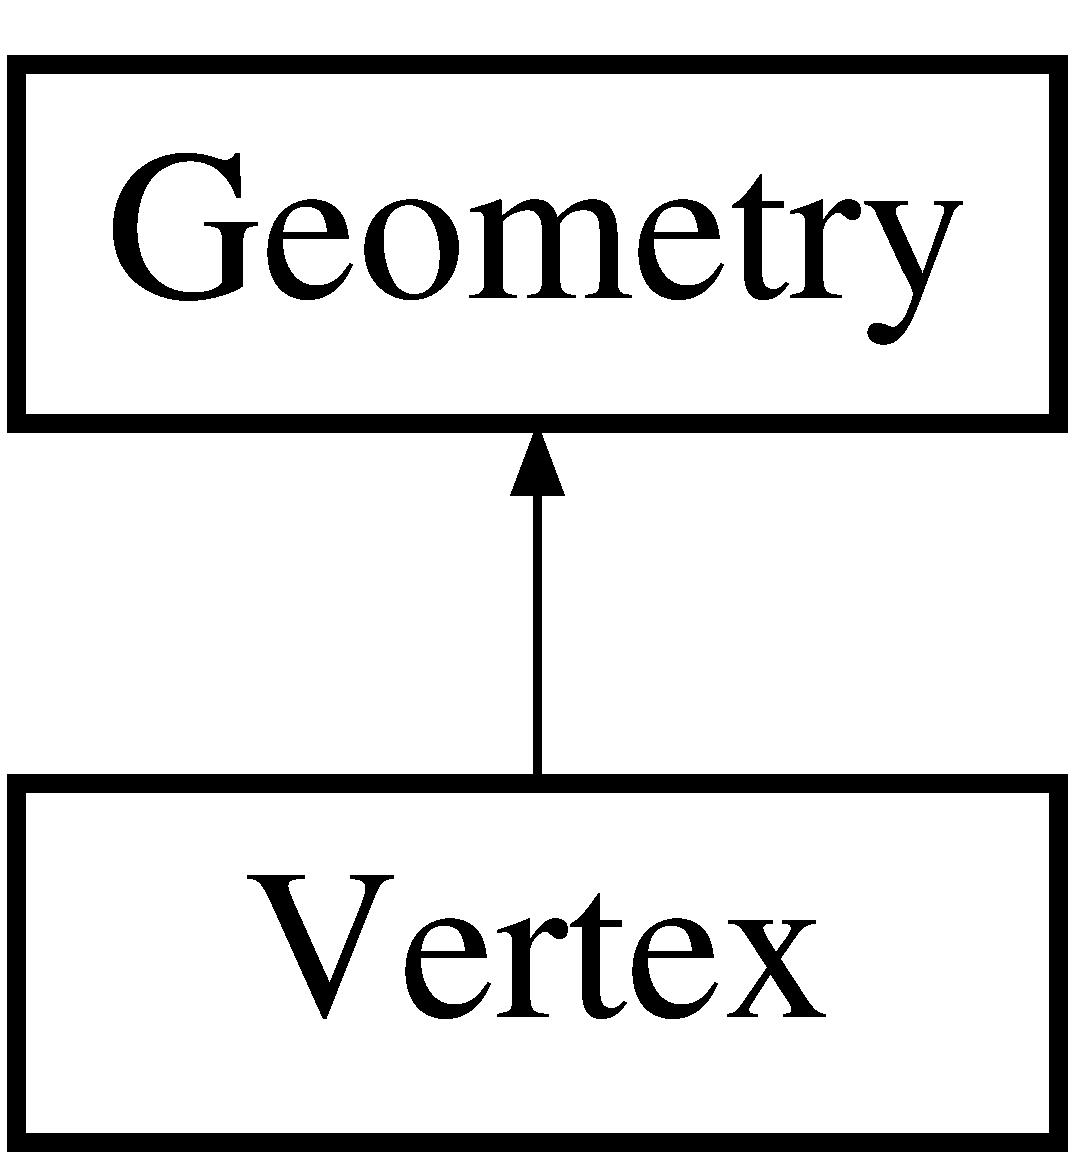
\includegraphics[height=2.000000cm]{class_vertex}
\end{center}
\end{figure}
\subsection*{Public Member Functions}
\begin{DoxyCompactItemize}
\item 
\hyperlink{class_vertex_a97488994a2482d70da74e1b91d40e169}{Vertex} ()
\item 
\hyperlink{class_vertex_a8531fa03e22d722369a91dc038467379}{Vertex} (\hyperlink{class_point3_d}{Point3D} point3d)
\item 
\hyperlink{class_vertex_ac3f28a791455bbd53724c8775c549b43}{Vertex} (double x, double y, double z)
\item 
void \hyperlink{class_vertex_afe14654ec1e3303294c53f4ed2a534f1}{Set\+Point} (\hyperlink{class_point3_d}{Point3D} point)
\item 
\hyperlink{class_point3_d}{Point3D} \hyperlink{class_vertex_a737ca423a44989a7dfc5ffa92e890781}{Get\+Point} () const
\end{DoxyCompactItemize}


\subsection{Detailed Description}
Class which provides internal application format for \textquotesingle{}vertex\textquotesingle{} structure. 

\subsection{Constructor \& Destructor Documentation}
\hypertarget{class_vertex_a97488994a2482d70da74e1b91d40e169}{}\label{class_vertex_a97488994a2482d70da74e1b91d40e169} 
\index{Vertex@{Vertex}!Vertex@{Vertex}}
\index{Vertex@{Vertex}!Vertex@{Vertex}}
\subsubsection{\texorpdfstring{Vertex()}{Vertex()}\hspace{0.1cm}{\footnotesize\ttfamily [1/3]}}
{\footnotesize\ttfamily Vertex\+::\+Vertex (\begin{DoxyParamCaption}{ }\end{DoxyParamCaption})}

Empty class constructor. \hypertarget{class_vertex_a8531fa03e22d722369a91dc038467379}{}\label{class_vertex_a8531fa03e22d722369a91dc038467379} 
\index{Vertex@{Vertex}!Vertex@{Vertex}}
\index{Vertex@{Vertex}!Vertex@{Vertex}}
\subsubsection{\texorpdfstring{Vertex()}{Vertex()}\hspace{0.1cm}{\footnotesize\ttfamily [2/3]}}
{\footnotesize\ttfamily Vertex\+::\+Vertex (\begin{DoxyParamCaption}\item[{\hyperlink{class_point3_d}{Point3D}}]{point3d }\end{DoxyParamCaption})}

Class constructor with \hyperlink{class_point3_d}{Point3D} argument. 
\begin{DoxyParams}{Parameters}
{\em point3d} & point representing vertex \\
\hline
\end{DoxyParams}
\hypertarget{class_vertex_ac3f28a791455bbd53724c8775c549b43}{}\label{class_vertex_ac3f28a791455bbd53724c8775c549b43} 
\index{Vertex@{Vertex}!Vertex@{Vertex}}
\index{Vertex@{Vertex}!Vertex@{Vertex}}
\subsubsection{\texorpdfstring{Vertex()}{Vertex()}\hspace{0.1cm}{\footnotesize\ttfamily [3/3]}}
{\footnotesize\ttfamily Vertex\+::\+Vertex (\begin{DoxyParamCaption}\item[{double}]{x,  }\item[{double}]{y,  }\item[{double}]{z }\end{DoxyParamCaption})}

Class constructor with coordinates. Creates \hyperlink{class_point3_d}{Point3D} with given coordinates. 
\begin{DoxyParams}{Parameters}
{\em x} & the x coordinate \\
\hline
{\em y} & the y coordinate \\
\hline
{\em z} & the z coordinate \\
\hline
\end{DoxyParams}


\subsection{Member Function Documentation}
\hypertarget{class_vertex_a737ca423a44989a7dfc5ffa92e890781}{}\label{class_vertex_a737ca423a44989a7dfc5ffa92e890781} 
\index{Vertex@{Vertex}!Get\+Point@{Get\+Point}}
\index{Get\+Point@{Get\+Point}!Vertex@{Vertex}}
\subsubsection{\texorpdfstring{Get\+Point()}{GetPoint()}}
{\footnotesize\ttfamily \hyperlink{class_point3_d}{Point3D} Vertex\+::\+Get\+Point (\begin{DoxyParamCaption}{ }\end{DoxyParamCaption}) const}

Returns point representing vertex. \begin{DoxyReturn}{Returns}
point representing vertex 
\end{DoxyReturn}
\hypertarget{class_vertex_afe14654ec1e3303294c53f4ed2a534f1}{}\label{class_vertex_afe14654ec1e3303294c53f4ed2a534f1} 
\index{Vertex@{Vertex}!Set\+Point@{Set\+Point}}
\index{Set\+Point@{Set\+Point}!Vertex@{Vertex}}
\subsubsection{\texorpdfstring{Set\+Point()}{SetPoint()}}
{\footnotesize\ttfamily void Vertex\+::\+Set\+Point (\begin{DoxyParamCaption}\item[{\hyperlink{class_point3_d}{Point3D}}]{point }\end{DoxyParamCaption})}

Method sets point field of the object. 
\begin{DoxyParams}{Parameters}
{\em point} & point representing the vertex \\
\hline
\end{DoxyParams}


The documentation for this class was generated from the following file\+:\begin{DoxyCompactItemize}
\item 
include/Geometry.\+h\end{DoxyCompactItemize}

\hypertarget{class_windows_communication}{}\section{Windows\+Communication Class Reference}
\label{class_windows_communication}\index{Windows\+Communication@{Windows\+Communication}}
Inheritance diagram for Windows\+Communication\+:\begin{figure}[H]
\begin{center}
\leavevmode
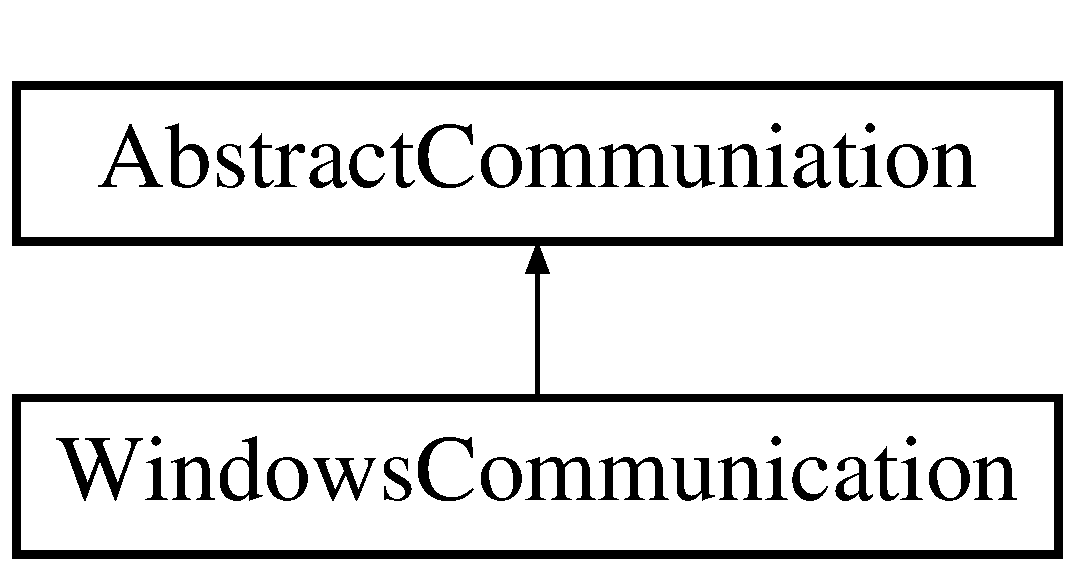
\includegraphics[height=2.000000cm]{class_windows_communication}
\end{center}
\end{figure}
\subsection*{Public Member Functions}
\begin{DoxyCompactItemize}
\item 
\hypertarget{class_windows_communication_aed89a58fa57d0bd0cc6d0342310977ce}{}\label{class_windows_communication_aed89a58fa57d0bd0cc6d0342310977ce} 
{\bfseries Windows\+Communication} (int port\+\_\+number)
\item 
\hypertarget{class_windows_communication_a18db3adb397e4c9036e39887485e0f32}{}\label{class_windows_communication_a18db3adb397e4c9036e39887485e0f32} 
void {\bfseries Setup\+Socket} ()
\item 
\hypertarget{class_windows_communication_a0e6b9db2e11a01ba976f2d1528e0b98f}{}\label{class_windows_communication_a0e6b9db2e11a01ba976f2d1528e0b98f} 
void {\bfseries Cleanup\+Socket} ()
\item 
\hypertarget{class_windows_communication_a8acfdac5781409bf6e563ea620ae6d3b}{}\label{class_windows_communication_a8acfdac5781409bf6e563ea620ae6d3b} 
int {\bfseries Send\+Bytes\+To\+Core} (const char $\ast$buffer, int buffer\+\_\+size) const
\item 
\hypertarget{class_windows_communication_a634009aa53f3737ee2612dcde51d081a}{}\label{class_windows_communication_a634009aa53f3737ee2612dcde51d081a} 
int {\bfseries Get\+Bytes\+From\+Core} (char $\ast$buffer, int buffer\+\_\+size)
\end{DoxyCompactItemize}
\subsection*{Additional Inherited Members}


The documentation for this class was generated from the following file\+:\begin{DoxyCompactItemize}
\item 
include/Windows\+Communication.\+h\end{DoxyCompactItemize}

%--- End generated contents ---

% Index
\backmatter
\newpage
\phantomsection
\clearemptydoublepage
\addcontentsline{toc}{chapter}{Index}
\printindex

\end{document}
